% ===============================================================
% LIST OF FILES 
% Lecture Notes  --  main file  (compile with pdfLaTeX)
%  Structure:
%     preamble/   packages, style, macros, boxes, code settings
%     sections/   one file per section of the lecture
%     figures/    TikZ / pgfplots figures (and put images here too)
%     code/       source files shown with \lstinputlisting
% ===============================================================
\documentclass[11pt,a4paper]{article}

% ----- Course metadata (edit these) -----
\newcommand{\coursecode}{Subject Code}
\newcommand{\coursename}{Subject Name}
\newcommand{\lecnumber}{1}
\newcommand{\lectitle}{Title of the Topic}
\newcommand{\lecturer}{Name of the Professor}
\newcommand{\semester}{Semester / Session}

% ----- Preamble (order matters: colors in style.tex are used by later files) -----
% ------------- For Encoding & fonts ----------------
\usepackage[T1]{fontenc}
\usepackage[utf8]{inputenc}
\usepackage{lmodern}
\usepackage[scaled=.92]{helvet}   % sans-serif for headings
\usepackage{microtype}

% ---------------- For Layout ----------------
\usepackage[margin=1in, headheight=15pt]{geometry}
\usepackage{setspace}
\setstretch{1.1}
\usepackage{enumitem}
\setlist{itemsep=2pt, topsep=4pt}
\usepackage{booktabs, array, graphicx}
\usepackage{caption, subcaption}
\captionsetup{font=small, labelfont={bf,sf}, format=hang}

% ---------------- For Color ----------------
\usepackage[dvipsnames,svgnames]{xcolor}

% ---------------- For Math ----------------
\usepackage{amsmath, amssymb, amsthm, mathtools, bm}

% ---------------- For Boxes ----------------
\usepackage[most]{tcolorbox}

% ------------- For Code & algorithms ----------------
\usepackage{listings}
\usepackage{algorithm}
\usepackage[noend]{algpseudocode}

% -------------- For Figures / plots ----------------
\usepackage{tikz}
\usetikzlibrary{arrows.meta, positioning, shapes.geometric, calc, fit, backgrounds}
\usepackage{pgfplots}
\pgfplotsset{compat=newest}

% ------------- For Headings, headers ----------------
\usepackage{titlesec}
\usepackage{fancyhdr}
\usepackage{lastpage}

% -------- For Hyperlinks (load last) ----------------
\usepackage[colorlinks=true, linkcolor=accent, citecolor=accent3, urlcolor=accent2]{hyperref}

% ---------------- Colors (change the theme here) ----------------
\definecolor{accent}{HTML}{1F5FBF}     % main accent (blue)
\definecolor{accent2}{HTML}{C2410C}    % secondary accent (orange)
\definecolor{accent3}{HTML}{15803D}    % tertiary accent (green)
\definecolor{codebg}{HTML}{F6F8FA}
\definecolor{codegray}{HTML}{6A737D}
\definecolor{codekw}{HTML}{CF222E}
\definecolor{codestr}{HTML}{0A3069}
\definecolor{codefn}{HTML}{8250DF}

% ---------------- Section headings ----------------
\titleformat{\section}{\Large\sffamily\bfseries\color{accent}}{\thesection}{0.7em}{}
\titleformat{\subsection}{\large\sffamily\bfseries\color{black!80}}{\thesubsection}{0.7em}{}
\titleformat{\subsubsection}{\normalsize\sffamily\bfseries\color{black!70}}{\thesubsubsection}{0.7em}{}
\titlespacing*{\section}{0pt}{16pt}{8pt}

% ---------------- Header / footer ----------------
% \pagestyle{fancy}
% \fancyhf{}
% \fancyhead[L]{\sffamily\small\color{gray}\coursecode\ --- \coursename}
% \fancyhead[R]{\sffamily\small\color{gray}Lecture \lecnumber: \lectitle}
% \fancyfoot[C]{\sffamily\small\thepage}
% \renewcommand{\headrulewidth}{0.4pt}
% \renewcommand{\headrule}{\hbox to\headwidth{\color{gray!50}\leaders\hrule height \headrulewidth\hfill}}
\pagestyle{fancy}
\fancyhf{}
\fancyhead[L]{\sffamily\small\color{gray}\coursecode\ --- \coursename}
\fancyhead[R]{\sffamily\small\color{gray}Lecture \lecnumber: \lectitle}
\fancyfoot[L]{\sffamily\small\color{gray}\lecturer\ $\cdot$ \semester}
\fancyfoot[C]{\sffamily\small\color{gray}\coursecode}
\fancyfoot[R]{\sffamily\small\color{gray}Page \thepage\ of \pageref{LastPage}}
\renewcommand{\headrulewidth}{0.4pt}
\renewcommand{\footrulewidth}{0.4pt}
\renewcommand{\headrule}{\hbox to\headwidth{\color{gray!50}\leaders\hrule height \headrulewidth\hfill}}
\renewcommand{\footrule}{\hbox to\headwidth{\color{gray!50}\leaders\hrule height \footrulewidth\hfill}}

% ---------------- Title block ----------------
\newcommand{\makelecturetitle}{%
  \begin{tcolorbox}[enhanced, colback=accent, colframe=accent, coltext=white,
    sharp corners, boxrule=0pt, left=14pt, right=14pt, top=12pt, bottom=12pt,
    overlay={\fill[white,opacity=0.08] (frame.south east) circle (2.2cm);}]
    {\sffamily\small\textbf{\coursecode}\ $\cdot$\ \coursename\hfill \semester\par}
    \vspace{6pt}
    {\sffamily\bfseries\huge Lecture \lecnumber: \lectitle\par}
    \vspace{6pt}
    {\sffamily\small Lecturer: \lecturer\hfill Compiled: \today\par}
  \end{tcolorbox}
  \vspace{6pt}
}

% ---------------- Math macros ----------------
\newcommand{\R}{\mathbb{R}}
\newcommand{\N}{\mathbb{N}}
\newcommand{\Z}{\mathbb{Z}}
\newcommand{\E}{\mathbb{E}}
\renewcommand{\Pr}{\mathbb{P}}
% \O already exists in LaTeX (the letter O-slash), so keep it for text mode
% and use \mathcal{O} (Big-O) in math mode.
\let\oslashletter\O
\renewcommand{\O}{\ifmmode\mathcal{O}\else\oslashletter\fi}
\newcommand{\norm}[1]{\left\lVert #1 \right\rVert}
\newcommand{\abs}[1]{\left\lvert #1 \right\rvert}
\newcommand{\inner}[2]{\left\langle #1, #2 \right\rangle}
\DeclareMathOperator*{\argmin}{arg\,min}
\DeclareMathOperator*{\argmax}{arg\,max}

% Nicer QED symbol
\renewcommand{\qedsymbol}{$\blacksquare$}

% Inline code:  \code{merge\_sort(A)}
\newcommand{\code}[1]{\colorbox{codebg}{\texttt{\small #1}}}
% ---------------- Base style for all boxes ----------------
\tcbset{
  thmbase/.style={
    enhanced, breakable, sharp corners, boxrule=0pt, frame hidden,
    left=10pt, right=8pt, top=6pt, bottom=6pt,
    fonttitle=\sffamily\bfseries, before skip=10pt, after skip=10pt
  }
}

% ---------------- Numbered boxes ----------------
% Usage: \begin{theorem}{Title}{label} ... \end{theorem}   ref: Theorem~\ref{thm:label}
\newtcbtheorem[number within=section]{theorem}{Theorem}%
  {thmbase, colback=accent!6, borderline west={3pt}{0pt}{accent}, coltitle=accent}{thm}
\newtcbtheorem[use counter from=theorem]{lemma}{Lemma}%
  {thmbase, colback=accent!6, borderline west={3pt}{0pt}{accent}, coltitle=accent}{lem}
\newtcbtheorem[use counter from=theorem]{definition}{Definition}%
  {thmbase, colback=accent3!7, borderline west={3pt}{0pt}{accent3}, coltitle=accent3}{def}
\newtcbtheorem[use counter from=theorem]{example}{Example}%
  {thmbase, colback=accent2!6, borderline west={3pt}{0pt}{accent2}, coltitle=accent2}{ex}
\newtcbtheorem[number within=section]{exercise}{Exercise}%
  {thmbase, colback=gray!8, borderline west={3pt}{0pt}{gray}, coltitle=black!70}{exc}

% ---------------- Unnumbered boxes ----------------
\newtcolorbox{keyidea}[1][Key Idea]{thmbase, colback=yellow!12,
  borderline west={3pt}{0pt}{yellow!70!orange},
  before upper={\textbf{\sffamily\color{yellow!40!black}#1.}\ }}
\newtcolorbox{notebox}[1][Note]{thmbase, colback=gray!8,
  borderline west={3pt}{0pt}{gray!70},
  before upper={\textbf{\sffamily\color{black!70}#1.}\ }}
\newtcolorbox{warnbox}[1][Warning]{thmbase, colback=red!6,
  borderline west={3pt}{0pt}{red!70!black},
  before upper={\textbf{\sffamily\color{red!70!black}#1.}\ }}
\newtcolorbox{objectives}{thmbase, colback=accent!6,
  borderline west={3pt}{0pt}{accent},
  before upper={\textbf{\sffamily\color{accent}Learning objectives}\par\vspace{2pt}}}

% ---------------- Listings style ----------------
\lstdefinestyle{modern}{
  backgroundcolor=\color{codebg},
  basicstyle=\ttfamily\small,
  commentstyle=\itshape\color{codegray},
  keywordstyle=\bfseries\color{codekw},
  stringstyle=\color{codestr},
  identifierstyle=\color{black},
  numbers=left, numberstyle=\tiny\color{codegray}, numbersep=8pt,
  frame=lines, rulecolor=\color{gray!40},
  framexleftmargin=4pt, xleftmargin=14pt,
  breaklines=true, breakatwhitespace=true,
  postbreak=\mbox{\textcolor{codegray}{$\hookrightarrow$}\space},
  showstringspaces=false, tabsize=4, captionpos=b,
  aboveskip=10pt, belowskip=6pt
}
\lstset{style=modern}

% ---------------- Algorithm style ----------------
\algrenewcommand\algorithmicrequire{\textbf{Input:}}
\algrenewcommand\algorithmicensure{\textbf{Output:}}
\floatname{algorithm}{Algorithm}


\begin{document}

\makelecturetitle

\begin{objectives}
After this lecture you should be able to:
\begin{itemize}
  \item state and apply the divide-and-conquer paradigm;
  \item analyze recurrences using recursion trees and induction;
  \item implement merge sort and Dijkstra's algorithm.
\end{itemize}
\end{objectives}

\tableofcontents
\bigskip

\section{Introduction}
Divide and conquer solves a problem by splitting it into smaller subproblems,
solving them recursively, and combining the results. Inline math such as
$T(n) = 2T(n/2) + \O(n)$ and inline code such as \code{merge\_sort(A)}
sit comfortably together. Cross-references work as usual: see
Section~\ref{sec:math}, Algorithm~\ref{alg:dijkstra}, Listing~\ref{lst:merge},
and Figure~\ref{fig:graph}.

\begin{keyidea}[Key idea]
Many efficient algorithms follow one pattern: \emph{split}, \emph{recurse}, \emph{merge}.
The cost is determined by how the work at each level of the recursion adds up.
\end{keyidea}

\section{Mathematical Foundations}\label{sec:math}

\begin{definition}{Big-O notation}{bigo}
Let $f,g:\N\to\R_{\ge 0}$. We write $f(n)=\O(g(n))$ if there exist $c>0$ and
$n_0\in\N$ such that $f(n)\le c\,g(n)$ for all $n\ge n_0$.
\end{definition}

\begin{theorem}{Merge sort recurrence}{mergesort}
Let $T(n)=2T(n/2)+n$ with $T(1)=1$ for $n$ a power of two. Then
$T(n)=n\log_2 n + n=\Theta(n\log n)$.
\end{theorem}

\begin{proof}
We argue by induction on $k$ where $n=2^k$. For $k=0$, $T(1)=1=1\cdot 0+1$.
Assume the claim for $n/2$. Then
\begin{align}
T(n) &= 2\,T(n/2) + n \notag\\
     &= 2\left(\tfrac{n}{2}\log_2\tfrac{n}{2} + \tfrac{n}{2}\right) + n \notag\\
     &= n(\log_2 n - 1) + n + n \notag\\
     &= n\log_2 n + n. \qedhere
\end{align}
\end{proof}

\begin{example}{Gradient descent step}{gd}
For a differentiable $f:\R^d\to\R$ the update with step size $\eta>0$ is
\[
  \bm{x}_{t+1} = \bm{x}_t - \eta\,\nabla f(\bm{x}_t),
  \qquad
  \bm{x}^\star \in \argmin_{\bm{x}} f(\bm{x}).
\]
\end{example}

\begin{notebox}[Note]
Use \texttt{\textbackslash begin\{theorem\}\{Title\}\{label\}} and refer to it
with \texttt{Theorem~\textbackslash ref\{thm:label\}}. For instance,
Theorem~\ref{thm:mergesort} above.
\end{notebox}

A small table with \texttt{booktabs}:
\begin{table}[h]
\centering
\caption{Common running times.}
\begin{tabular}{@{}lll@{}}
\toprule
\textbf{Algorithm} & \textbf{Time} & \textbf{Space} \\
\midrule
Merge sort      & $\O(n\log n)$     & $\O(n)$ \\
Quicksort (avg) & $\O(n\log n)$     & $\O(\log n)$ \\
Dijkstra (heap) & $\O((V+E)\log V)$ & $\O(V)$ \\
\bottomrule
\end{tabular}
\end{table}

\section{Algorithms}

\begin{algorithm}[t]
\caption{Dijkstra's shortest paths}\label{alg:dijkstra}
\begin{algorithmic}[1]
\Require Graph $G=(V,E)$, weights $w:E\to\R_{\ge 0}$, source $s\in V$
\Ensure Shortest-path distances $d[v]$ from $s$ to every $v\in V$
\State $d[v]\gets\infty$ for all $v\in V$; \ $d[s]\gets 0$
\State $Q\gets$ priority queue containing all $v\in V$ keyed by $d[v]$
\While{$Q\neq\emptyset$}
  \State $u\gets$ \Call{ExtractMin}{$Q$}
  \ForAll{edges $(u,v)\in E$}
    \If{$d[u]+w(u,v)<d[v]$}
      \State $d[v]\gets d[u]+w(u,v)$
      \State \Call{DecreaseKey}{$Q,v,d[v]$}
    \EndIf
  \EndFor
\EndWhile
\State \Return $d$
\end{algorithmic}
\end{algorithm}

\begin{lemma}{Correctness invariant}{inv}
When a vertex $u$ is extracted from $Q$, $d[u]$ equals the true shortest-path
distance $\delta(s,u)$.
\end{lemma}

\section{Code}

% Source files live in code/ -- edit them there and they update here.
\lstinputlisting[language=Python, caption={Merge sort in Python.}, label={lst:merge}]{code/merge_sort.py}

\lstinputlisting[language=C++, caption={Binary search in C++.}, label={lst:bsearch}]{code/binary_search.cpp}

% Short snippets can also be written inline:
% \begin{lstlisting}[language=Python, caption={...}, label={lst:x}]
% print("hello")
% \end{lstlisting}

\begin{warnbox}[Pitfall]
Writing \code{(lo + hi) / 2} can overflow for large indices; use
\code{lo + (hi - lo) / 2} as in Listing~\ref{lst:bsearch}.
\end{warnbox}

\section{Figures and Plots}

\begin{figure}[h]
\centering
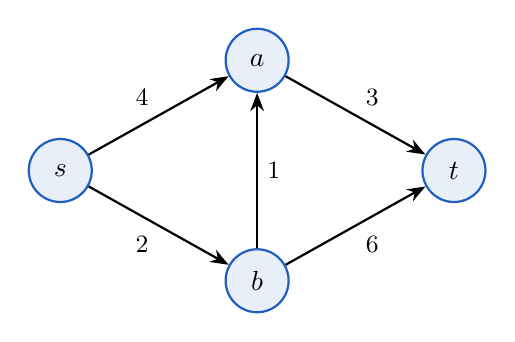
\begin{tikzpicture}[
  >=Stealth, thick,
  v/.style={circle, draw=accent, fill=accent!10, minimum size=8mm, font=\sffamily}
]
  \node[v] (s) at (0,0)     {$s$};
  \node[v] (a) at (2.5,1.4) {$a$};
  \node[v] (b) at (2.5,-1.4){$b$};
  \node[v] (t) at (5,0)     {$t$};
  \draw[->] (s) -- node[above left]  {\small 4} (a);
  \draw[->] (s) -- node[below left]  {\small 2} (b);
  \draw[->] (a) -- node[above right] {\small 3} (t);
  \draw[->] (b) -- node[below right] {\small 6} (t);
  \draw[->] (b) -- node[right]       {\small 1} (a);
\end{tikzpicture}

\caption{A small weighted digraph. The shortest $s$--$t$ path is $s\to b\to a\to t$ with cost $6$.}
\label{fig:graph}
\end{figure}

\begin{figure}[h]
\centering
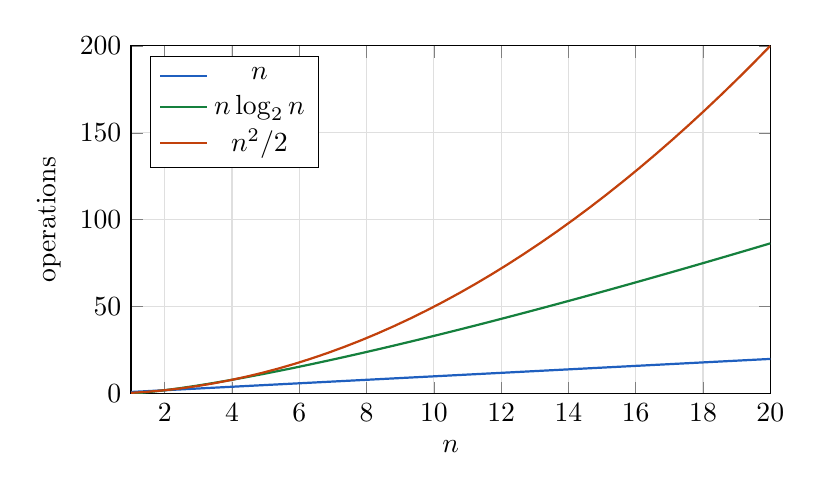
\begin{tikzpicture}
\begin{axis}[
  width=0.8\linewidth, height=6cm,
  xlabel={$n$}, ylabel={operations},
  xmin=1, xmax=20, ymin=0, ymax=200,
  legend pos=north west, grid=major, grid style={gray!25},
  every axis plot/.append style={thick}
]
  \addplot[accent,  domain=1:20, samples=40] {x};
  \addplot[accent3, domain=1:20, samples=40] {x*ln(x)/ln(2)};
  \addplot[accent2, domain=1:20, samples=40] {x^2/2};
  \legend{$n$, $n\log_2 n$, $n^2/2$}
\end{axis}
\end{tikzpicture}

\caption{Growth rates of common running times.}
\label{fig:growth}
\end{figure}

% To include an external image (upload it to figures/ first):
% \begin{figure}[h]
%   \centering
%   \includegraphics[width=0.6\linewidth]{figures/my_diagram.pdf}
%   \caption{Caption here.}
% \end{figure}

\section{Exercises}

\begin{exercise}{Recurrence}{rec}
Solve $T(n)=3T(n/2)+n$ with $T(1)=1$ using a recursion tree, and give a tight
$\Theta$-bound.
\end{exercise}

\begin{exercise}{Implementation}{impl}
Modify Listing~\ref{lst:merge} to count the number of inversions in $\O(n\log n)$ time.
\end{exercise}

\section*{Further Reading}
\begin{itemize}
  \item T.~Cormen, C.~Leiserson, R.~Rivest, C.~Stein. \emph{Introduction to Algorithms}, MIT Press.
  \item J.~Kleinberg, \'E.~Tardos. \emph{Algorithm Design}, Pearson.
\end{itemize}


\end{document}
